\chapter{强化学习算法研究与分析}\label{rl}

\section{强化学习基本原理}
强化学习的本质是通过与环境的交互进行学习。强化学习智能体与环境进行交互,并在观察到其行为的结果时,通过学习来改变自己的行为方式以响应所获得的奖励或惩罚。这种试错学习方法的范式来源于行为主义心理学,是强化学习的主要基础之一\cite{17}。另一个影响了强化学习的关键思想史最优控制,它提供了支撑该领域的数学形式。

在强化学习过程中,有机器学习算法控制的自主智能体在$t$时刻从环境中观察到状态$s_t$。智能体通过在状态$s_t$中执行动作$a_t$来与环境交互。当智能体执行动作时,环境和智能体将会根据当前的状态和所选择的动作转移到新的状态$s_{t+1}$。状态是对环境的充分统计数据,因此包括智能体采取最佳动作的所有必要信息,比如轮式机器人在环境中的位置。

最佳的动作顺序取决于环境提供的奖励。每次环境转换到新的状态时,它还会向智能体提供一个标量奖励$r_{t+1}$作为反馈。智能体的目标是学习一种最大化预期累加折扣的回报的策略。给定一个状态,策略返回要执行的动作,最优的策略就是能够最大化环境预期回报的策略。在这方面,强化学习旨在解决与最优控制相同的问题。然而,不像最优控制模型,强化学习中挑战的是智能体在不能获得状态转移的模型的情况下,通过反复试验来了解环境中行为的后果。与环境的每次交互都会产生信息,智能体会使用这些信息来更新其知识。这种感知、动作、学习的循环如图\ref{stateaction}所示。
\begin{figure}[htb]
  \centering
  % Requires \usepackage{graphicx}
  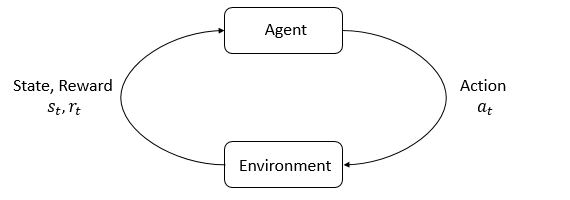
\includegraphics[width=0.80\textwidth]{figures/stateaction.png}
  \caption{强化学习基本模型}\label{stateaction}
\end{figure}

\subsection{马尔可夫决策过程}
强化学习过程可以用马尔可夫决策过程(MDP, Markov Decision Process)描述,它包含了以下定义:
\begin{itemize}
  \item $\mathcal{S}$,状态集合,包含一个初始状态分布$p \left( s_0 \right)$。
  \item $\mathcal{A}$,动作集合。
  \item $\mathcal{T}(s_{t+1}|s_t,a_t)$,状态转移函数,从$t$时刻的状态-动作对映射到$t+1$时的状态分布。
  \item $\mathcal{R}(s_t, a_t, s_{t+1})$,瞬时奖励。
  \item $\gamma \in [0,1]$,折扣参数,较低的折扣参数就会使模型更加重视瞬时奖励,较高的折扣参数则会使模型更加重视长期奖励。
\end{itemize}

通常来说,策略$\pi$定义了在特定时间特定状态下的行为方式,是一个从状态到每个可能的动作的概率的映射:$\pi : \mathcal{S} \to p(\mathcal{A} = a | \mathcal{S})$。$\pi(a_t|s_t)$就是指在状态$s_t$时选择执行动作$a_t$的概率。

在马尔可夫决策过程中,一个智能体从初始状态$s_0 \in \mathcal{S}$开始,在$t$时刻,观察到状态$s_t$,根据策略$\pi(a|s_t)$选择一个动作$a_t \in \mathcal{A}$执行,同时根据状态转移函数$\mathcal{T}(s|s_t,a_t)$,改变了智能体在环境中的状态到$s_{t+1} \in \mathcal{S}$,并使智能体获得奖励$r = \mathcal{R}(s_t, a_t, s_{t+1})$。z这一过程,如图\ref{mdp} 所示。

\begin{figure}[htb]
  \centering
  % Requires \usepackage{graphicx}
  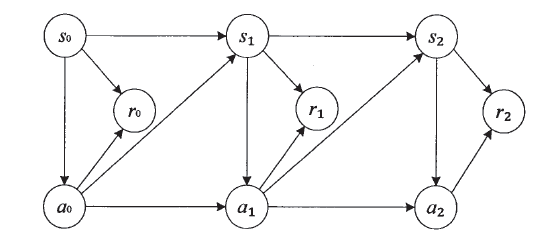
\includegraphics[width=0.80\textwidth]{figures/mdp.png}
  \caption{MDP动态过程}\label{mdp}
\end{figure}

对于情节性任务(Episodic Task),指状态会在时间$T$后结束并重置,以自然结束智能体(agent)和环境(environment)的交互,即所有任务可以被分解成一系列情节(episode),而情节的数目是有限的。那么在每一个情节中,状态、动作和奖励的序列就组成一个轨迹(trajectory)。一种策略中每一个轨迹所对应的瞬时奖励的折扣累加就是这个轨迹的回报(return)。
\begin{equation}
R = \sum_{k=0}^{T-1} \gamma^t r_{t+1}.
\end{equation}

对于连续性任务(Continuing Task),指任务不会自然结束,会一直持续到$T = \infty$。在这种情况下,我们使用$\gamma < 1$以保证累加奖励趋向于无穷。对于这种情况,我们不能计算一个完整轨迹的返回值,而是使用轨迹的一个有限子集。

强化学习的目标就是找到一个最优策略$\pi*$以最大化回报的期望。
\begin{equation}
\pi* = \text{argmax}_\pi \Bbb{E}[R|\pi].
\end{equation}

对于基于马尔可夫决策过程理论的强化学习来说,有一个重要的概念,那就是只有当前的状态会影响下一个状态,换而言之,在给定当前状态的情况下,未来状态与过去的状态是条件无关的。这意味着在状态$s_t$做出的任何动作决策只依赖于前一状态$s_{t-1}$\cite{18},而非${s_0, s_1, ..., s_{t-1}}$。即使这一假设被大多数强化学习方法采纳,但是这在本次实验的真实环境下是不现实的。因为这要求智能体的状态是能够被完全观察到的。

实际上当处于真实环境下,轮式机器人智能体只能观察到真实世界的部分状态。因此使用与马尔可夫决策过程的一般情况,部分可观测马尔可夫决策过程(POMDP)。在部分可观测马尔可夫决策过程中,智能体接收到一个观察结果(observation)$o_t \in \Omega$。观察结果是一个依赖于当前状态和先前动作的概率分布:$p(\o_{t+1}|s_{t+1},a_t)$。

在给定先前置信状态,采取的动作和当前的观察状态下,部分可观测马尔可夫决策过程通常维护一个对当前状态的置信度。深度学习中更常见的方法是利用递归神经网络(RNN, Recurrent Neural Network)。 它与前馈神经网络不同,是一个动态系统。当真实状态无法获知只能估计时,这种方法通过动态系统和状态空间模型解决了部分可观测马尔可夫决策过程。

\section{强化学习算法}
目前强化学习面临着许多挑战:
\begin{itemize}
  \item 强化学习必须通过与环境的反复实验来推断最优策略。智能体收到的唯一学习信号是奖励。
  \item 智能体的观察取决于其行为并且很可能包含强时间相关性。
  \item 智能体必须处理长时间的依赖关系。通常,一个动作的后果在环境状态进行多次转移后才会显现。
\end{itemize}

以轮式机器人你自主决策作战为例。如果目标位置已经确定,我们可能能够估计剩余的距离,并将其作为奖励信号,但我们不太可能确切地知道轮式机器人需要采取什么样的动作序列才能达到目标。由于轮式机器人必须在做出行进目标决策的同时导航,它的决策影响了它所能感知到的状态空间。最后,在导航了几个交叉路口后,轮式机器人可能会发现自己处于一条死路。从学习动作的后果到平衡探索与实践之间存在一系列问题,但这最终都可以来强化学习框架内解决。

根据是否基于模型,可以将强化学习算法分为基于模型学习(model-based learning)和模型无关学习(model-free learning)两种。

我们定义智能体学习和优化的策略称为目标策略,把智能体与环境进行实际交互行为的策略称为行为策略。根据智能体学习到的目标策略与智能体与实际环境交互的行为策略是否相同,我们将智能体分为同步策略学习(on-policy learning),又称在线学习和异步策略学习(off-policy learning),又称离线学习两种。

解决强化学习问题的方法主要分为两种:基于值函数的强化学习和基于策略搜索的强化学习。同时也有两种方法的混合,基于演员-评论家(actor-critic)模型的强化学习。

\subsection{值函数}
值函数方法基于估计所处状态的回报期望。状态值函数$V^{\pi}(s)$描述了处于状态$s$时,后续采取策略$\pi$的回报期望:
\begin{equation}
V^{\pi}(s) = \Bbb{E}[R|s,\pi].
\end{equation}

最优策略$\pi^*$对应的值函数$V*(s)$就是相应的最优值函数:
\begin{equation}
V^*(s) = \max_\pi V^{\pi}(s) \forall s \in \mathcal{S}.
\end{equation}

如果我们已经得到最优的值函数$V^*(s)$,最优策略$\pi^*$就可以通过回溯法得到。当智能体处于状态$s_t$时,在所有当前可以选择的动作中选择一个动作$a$最大化$\Bbb{E} _{s_{t+1} \sim \mathcal{T}(s_{t+1}|s_t,a)} [V^*(s_{t+1})]$。

在强化学习的过程中,状态转移函数$\mathcal{T}$是不可得的。因此,我们构建状态动作值函数$Q^\pi (s,a)$,即Q函数:
\begin{equation}
Q^{\pi}(s, a) = \Bbb{E} [R | s, a, \pi]
\end{equation}

在给定Q函数的情况下,最优策略可以通过在每一个状态下贪心选择动作$a = \text{argmax}_a Q^{\pi}(s, a)$来找到。在这种情况下,我们也可以定义$V^{\pi}(s)$,即$V^{\pi}(s) = \max_a Q^\pi (s,a)$。

为了实际学习$Q^\pi$,我们利用马尔可夫属性并将函数定义为Bellman方程,其具有以下递归形式:
\begin{equation}
Q^{\pi}(s_t, a_t) = \Bbb{E} [r_{t+1} + \gamma Q^\pi (s_{t+1}, \pi(s_{t+1}))].
\end{equation}

这意味着可以通过自助法(Bootstrapping)来优化$Q^\pi$,即我们可以使用对$Q^\pi$的估计的当前值来改进我们的估计。这是Q-learning\cite{19}和SARSA\cite{20}等算法的基础。

对于off-policy的Q-learning算法有:
\begin{equation}
Q^{\pi}(s_t, a_t) \leftarrow Q^{\pi}(s_t, a_t) + \alpha (r_t + \gamma \max_a Q^{\pi}(s_{t+1}, a)).
\end{equation}

对于on-policy的SARSA算法有:
\begin{equation}
Q^{\pi}(s_t, a_t) \leftarrow Q^{\pi}(s_t, a_t) + \alpha (r_t + \gamma Q^{\pi}(s_{t+1}, a_{t+1})).
\end{equation}

为了从任意$Q^\pi$中找到最优$Q^*$,我们使用广义策略迭代,其中策略迭代包括策略评估和策略改进。策略评估改进了值函数的估计,这可以通过最小化根据当前策略采取的路径产生的TD误差来实现。随着估计的改进,通过基于更新的值函数贪婪地选择动作,自然可以改善策略。通用策略迭代允许交错步骤,而不是单独地执行这些步骤以进行收敛,从而可以更快地进行。

\subsection{策略搜索}
策略搜索方法不需要维护值函数模型,而是直接搜索最优策略。通常选择参数化策略,之后使用基于梯度或无梯度的更新优化这些参数来最大化回报期望。使用神经网络对策略进行编码已经成功适用于无梯度和基于梯度的训练方法。无梯度优化可以有效地覆盖低维参数空间,尽管它们在应用于大型网络方面取得了一些成功\cite{21},但基于梯度的训练仍然是大多数深度强化学习的首选方法。当策略拥有大量参数时,基于梯度的训练的样本效率更高。

在直接构造策略时,通常输出概率分布的参数; 对于连续动作,这可以是高斯分布的均值和标准偏差,而对于离散动作,这可以是多项分布的个体概率。这样做的结果是一个可以直接采样动作的随机策略。使用无梯度方法,优化的策略则需要在预定义的模型类中进行启发式搜索。

\textbf{策略梯度(Policy Gradients):}对于如何改进参数化策略,梯度可以提供强有力的学习信号。然而,为了计算回报期望,我们需要对当前策略参数化引入的合理轨迹进行平均。这种平均需要确定性近似或通过采样的随机近似\cite{22}。确定性近似只能应用于基于模型的算法,其中可以获得状态转移函数的模型。在更常见的模型无关的R强化学习算法中,通常使用蒙塔卡罗方法估计回报期望。对于基于梯度的学习,这种蒙特卡罗近似提出了挑战,因为梯度不能通过随机函数的这些样本。因此,我们转向梯度的估计量,在强化学习中称为REINFORCE规则\cite{23}。REINFORCE规则可以用于计算随机变量$X$ 的函数$f$ 对于参数$\theta$ 的期望梯度:
\begin{equation}
\nabla_\theta \Bbb{E}_X [f(X;\theta)] = \Bbb{E}_X [f(X;\theta) \nabla_\theta \log p(X)].
\end{equation}

由于该计算依赖于轨迹的经验回归,因此得到的梯度具有高方差。通过引入噪声较小的无偏估计,可以减少方差。执行此操作的一般方法是减去基线,这意味着通过优势而不是纯回报来加权更新。

\textbf{演员-评论家(Actor-critic):}可以将值函数与策略的2显示表示相结合,从而产生演员-评论家方法,如图\ref{ac}所示。“演员”(策略)通过使用“评论家”(值函数)的反馈来学习。在这样做时,这些方法通过值函数方法的偏差引入来权衡策略梯度的方差减少\cite{23}\cite{24}。

演员-评论家方法使用值函数作为策略梯度的基线,因此演员-评论家方法与其他基线方法之间唯一的根本区别在于演员-评论家方法利用了一个优化过的值函数。
\begin{figure}[htb]
  \centering
  % Requires \usepackage{graphicx}
  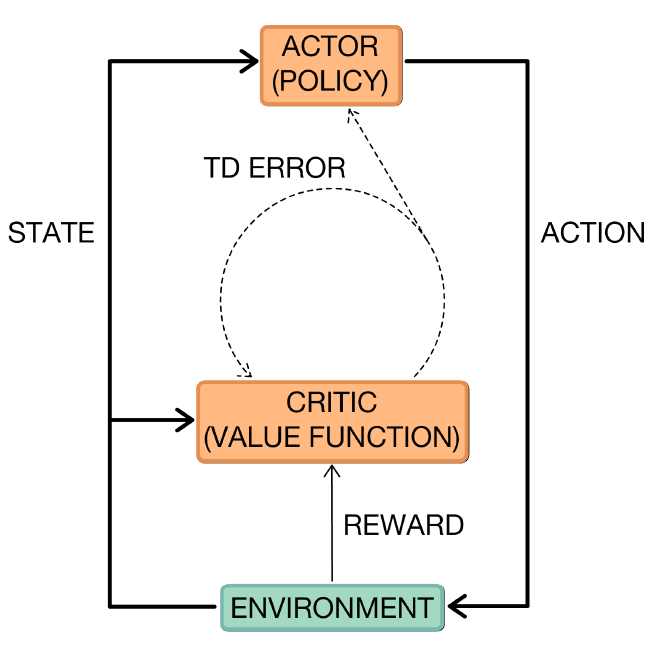
\includegraphics[width=0.80\textwidth]{figures/ac.png}
  \caption{演员-评论家(Actor-critic)方法}\label{ac}
\end{figure}

\subsection{深度强化学习}
深度强化学习的许多成功都是基于将强化学习的先前工作扩展到高维问题。这归功于低维特征学习和神经网络的强大函数逼近特性。通过特征学习,深度强化学习可以有效地处理维度灾难。例如,卷积神经网络(CNN, Convolutional Neural Network)可以用作强化学习智能体的组件,允许它们直接从原始的高维视觉输入中学习。通常,深度强化学习通过训练神经网络以近似最优策略$\pi^*$,或者最优值函数$V^*$,$Q^*$。

尽管当前深度强化学习成功使用无梯度的方法,但是绝大多数当前的工作依赖于梯度的反向传播算法。当可用时,梯度能够提供强大的学习信号。实际上,这些梯度是基于近似,通过采样或其他方式估计的,因此我们必须设计具有有效的归纳偏差的算法,以使它们易于处理。

反向传播的另一个好处是将回报期望的优化是为随机函数的优化。这个函数可以包含多个部分,包括模型、策略和值函数,通过各种方式组合。单个部分,例如值函数,可能不会直接优化回报期望,而是可以体现强化学习领域的有用信息。例如,使用可区分的模型和策略,可以在整个过程中进行前向传播和后向传播;另一方面,不确定性可能在很长一段时间内累积,此时使用值函数来总结统计数据可能是恰当的。我们之前已经提到特征学习和函数逼近是深度强化学习成功的关键,但也可以说深度学习领域激发了对强化学习的新思维方式。

\section{深度强化学习算法}
深度强化学习已经准备好在AI领域掀起一场革命。深度强化学习向建立对于真实世界具有高水平理解能力的全自主系统迈出了坚实的一步。当前,深度学习使强化学习有能力处理先前极为棘手的问题。深度强化学习也同样应用于机器人学领域,能够直接从真实世界摄像头的图片输入学习机器人控制策略。在本文中,我们首先介绍强化学习的通常概念,之后进一步阐述基于值和基于策略的方法。本文将覆盖深度强化学习的核心算法,包括DQN\cite{11}、DDPG\cite{26}、异步DDPG\cite{27}。同时,我们强调使用深度神经网络的优势,着重于关注于强化学习的理解。

\subsection{Deep Q-learning}
Deep Q-learning是第一个将深度学习模型与强化学习结合在一起从而成功地直接从高维的输入学习控制策略的算法。在Q-learning中使用Q值表来存储状态-动作对相应的Q值。然而当状态和动作空间是高维连续时,使用Q值表则不切实际。解决方法就是利用值函数近似,通过函数来近似Q值分布。借助深度神经网络来表示这个Q值函数就是DQN的核心思想。

通常DQN的实现中,会把收集的状态、动作、执行动作后的状态和奖励等信息存在内存中,训练的时候多次使用,称为回放记忆(replay memory)。注意到每个状态-动作对的Q值都要拟合,一个函数拟合自己可能引入额外的噪声,所以通常使用一个延迟更新的函数Q'来求新的Q值,称为目标值网络(target network),如图\ref{dqn}所示。如算法\ref{dqnalgorithm}所示。

DQN的改进包括Double DQN\cite{28}、Dueling DQN\cite{29}和Prioritized Replay\cite{30}。
Double DQN是在引入了target network后,改进Q值的计算方法,目的是减少因为Max Q值计算带来的计算偏差,或者称为过度估计问题。考虑到Q值和状态,动作都相关,但我们实际上更注重动作带来的奖励,Dueling DQN对网络结构做了改进。Prioritized Replay 探讨在回访记忆采样的优先级问题。

DQN以端到端的训练方式开创了深度强化学习对于高维输入的控制策略问题的解决方案。通过回放记忆解决相关性及非静态分布问题,使用目标值网络解决稳定性问题。但其在处理长时间的动作序列问题上仍然存在问题。

\begin{figure}[htb]
  \centering
  % Requires \usepackage{graphicx}
  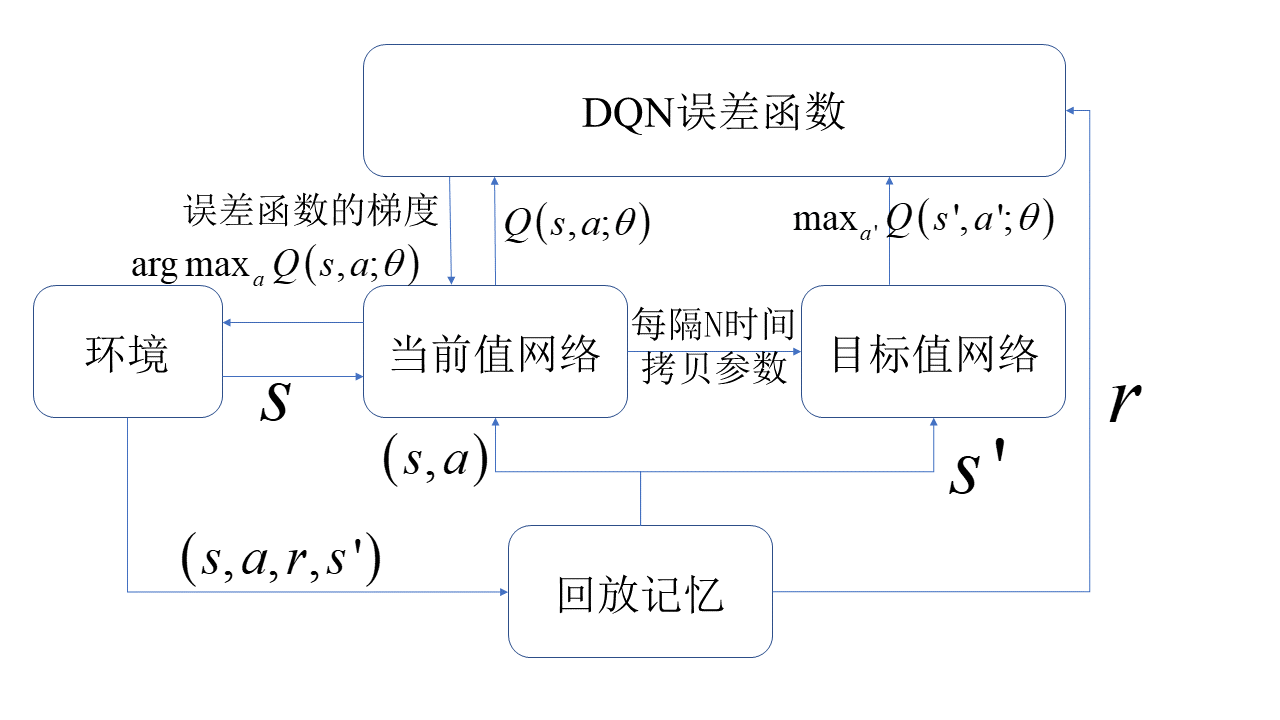
\includegraphics[width=\textwidth]{figures/DQN.png}
  \caption{DQN算法流程图}\label{dqn}
\end{figure}

\begin{algorithm}[htb]
\caption{Deep Q-learning}
\label{dqnalgorithm}
\begin{algorithmic}[1]
\State 初始化容量为$N$的回访记忆$\mathcal{D}$
\State 随机初始化动作值函数$Q$
\For{$\text{episode} = 1,M $}
    \State 初始化状态$s_1$
    \For{$t = 1, T$}
        \State 以概率$\epsilon$选择一个随机动作$a_t$
        \State 否则选择动作$a_t = \max_a Q^*(s_t,a;\theta)$
        \State 执行动作$a_t$得到奖励$r_t$并观察到环境$s_{t+1}$
        \State 保存$(s_t, a_t, r_t, s_{t+1})$到回放记忆$\mathcal{D}$
        \State 从回放记忆中采样一个minibatch$(s_t, a_t, r_t, s_{t+1})$
        \State 计算$y_j = \begin{cases} r_j,  & \text{$s_j$为终止状态} \\ r_j + \gamma \max_{a'} Q(s_{j+1}, a'; \theta), & \text{$s_{j+1}$不为终止状态}. \end{cases}$
        \State 计算$(y_j - Q(s_j, a_j; \theta))^2$的梯度下降并反向传播
    \EndFor
\EndFor
\end{algorithmic}
\end{algorithm}

\subsection{Deep Deterministic Policy Gradient}
深度确定性策略梯度(DDPG, Deep Deterministic Policy Gradient)是利用DQN扩展Q-learning算法的思路,对确定性策略梯度方法进行改造,基于前述演员-评论家框架的算法。该算法可用于解决连续动作空间上的深度强化学习问题。

DDPG中第一个D是深度神经网络,当概率策略的方差趋近于0的时候,就是确定性策略,其运用了Actor-Critic框架,把DQN和策略梯度混合了起来,显著提高样本利用率。如果动作空间也是连续的,那么就无法直接取到最大的Q值,那么我们再用个深度学习网络,称为演员Actor,演员的任务就是选Q值大的动作(确定性策略),演员的梯度来自值函数的估计网络(评论家),这个做法的最大优势是,能够离线地更新策略,即像DQN一样,从回放记忆采样出数据来训练,如图\ref{ddpg}所示。区别于DQN,DQN每隔一定的迭代次数后,将参数复制给实现网络;而DDPG中目标网络的参数每次迭代都以微小量逼近实现网络的参数。

在DDPG中,分别使用参数为$\theta^\mu$和$\theta^Q$的深度神经网络来表示确定性策略$a = \pi(s|\theta^\mu)$和动作值函数$Q(s,a|\theta^Q)$。其中,策略网络用来更新策略,对应演员;智网络用来逼近状态动作对的值函数,并提供梯度信息,对应评论家。目标函数被定义为带折扣的回报期望。
\begin{equation}
J(\theta^\mu) = \Bbb{E}_{\theta^\mu}[\sum_{t=0}^T \gamma^t r_{t+1}].
\end{equation}

通过随机梯度法对目标函数进行端到端的优化。目标函数关于$\theta^\mu$的梯度等价于Q值函数关于$\theta^\mu$的期望梯度:
\begin{equation}
\frac{\partial J(\theta^\mu)} {\partial \theta^\mu} = \Bbb{E}_s[\frac{\partial Q(s, a | \theta^Q)}{\partial \theta^\mu}].
\end{equation}

根据确定性策略$a = \pi(s|\theta^\mu)$,可得
\begin{equation}
\frac{\partial J(\theta^\mu)} {\partial \theta^\mu} = \Bbb{E}_s[\frac{\partial Q(s, a | \theta^Q)}{\partial a}\frac{\partial \pi(s|\theta^\mu)}{\partial \theta^\mu}].
\end{equation}

沿着提升Q值的方向更新策略网络的参数。

通过DQN中更新网络的方式来更新评论家网络,梯度信息为:
\begin{equation}
\frac{\partial L(\theta^Q)} {\partial \theta^Q} = \Bbb{E}_{s,a,r,s' \sim \mathcal{D}} [(r + \gamma Q'(s',\pi(s'|\theta^{\mu'})|\theta^{Q'}) - Q(s,a|\theta^Q)) \frac{\partial Q(s,a|\theta^Q)}{\partial \theta^Q}]
\end{equation}

如算法\ref{ddpgalgorithm}所示。

\begin{figure}[htb]
  \centering
  % Requires \usepackage{graphicx}
  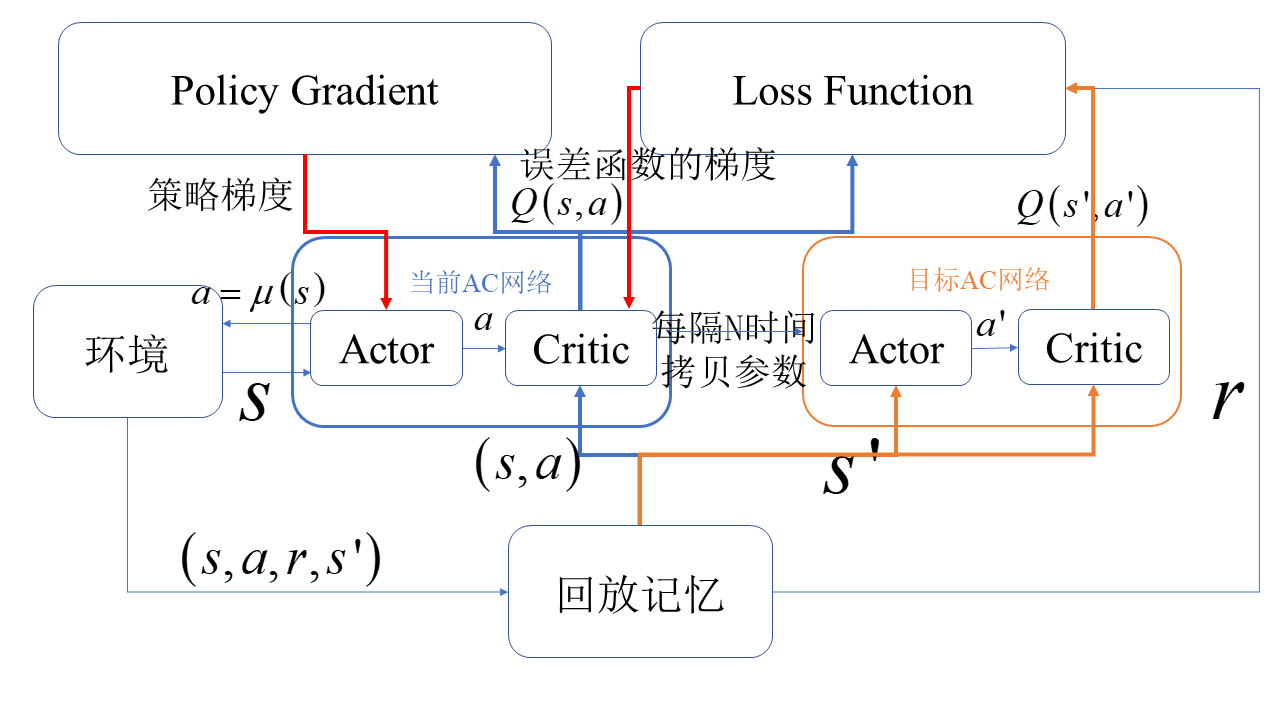
\includegraphics[width=\textwidth]{figures/ddpg.png}
  \caption{DDPG算法流程图}\label{ddpg}
\end{figure}

\begin{algorithm}[htb]
\caption{Deep Deterministic Policy Gradient}
\label{ddpgalgorithm}
\begin{algorithmic}[1]
\State 以随机参数$\theta^Q$和$\theta^\mu$初始化评论家网络$Q(s,a|\theta^Q)$和演员策略$\mu(s|\theta^\mu)$
\State 初始化容量为$N$的回访记忆$\mathcal{D}$
\For{$\text{episode} = 1,M $}
    \State 初始化状态$s_1$
    \State 初始化一个计算过程$\mathcal{N}$
    \For{$t = 1, T$}
        \State 选择动作$a_t = \mu(s_t|\theta^\mu) + \mathcal{N}_t$
        \State 执行动作$a_t$得到奖励$r_t$并观察到环境$s_{t+1}$
        \State 保存$(s_t, a_t, r_t, s_{t+1})$到回放记忆$\mathcal{D}$
        \State 从回放记忆中采样一个minibatch$(s_t, a_t, r_t, s_{t+1})$
        \State 计算$y_j = \begin{cases} r_j,  & \text{$s_j$为终止状态} \\ r_j + \gamma Q(s_{j+1}, \mu'(s_{i+1}|\theta^{\mu'}); \theta^{Q'}), & \text{$s_{j+1}$不为终止状态}. \end{cases}$
        \State 减小损失以更新评论家:$L = \frac{1}{N}\sum_j ((y_j - Q(s_j, a_j; \theta^Q))^2)$
        \State 使用策略梯度以更新演员:$\nabla_{\theta^\mu} J \approx \frac{1}{N} \sum_i \nabla_a Q(s,a|\theta^Q)|_{s=s_i,a=\mu(s_i)} \nabla_{\theta^\mu} \mu(s|\theta^\mu)$
    \EndFor
\EndFor
\end{algorithmic}
\end{algorithm}

DDPG不仅在一系列连续动作空间的任务中表现稳定,而且求得最优解所需要的时间步也远远少于DQN。与基于值函数的深度强化学习方法相比,基于演员-评论家框架的深度策略梯度方法优化策略效率更高,求解速度更快。

\subsection{多智能体异步DDPG}
与虚拟环境相比,在真实环境中,深度强化学习在轮式机器人上的训练面临以下挑战:
\begin{itemize}
  \item 在虚拟环境下训练深度强化学习时,可以通过读取一帧状态后暂停模拟器,训练网络后再启动模拟器执行动作。而在真实环境下的轮式机器人控制是一个要求强实时性的问题。当读取一帧状态还未选择动作时,状态可能已经发生了变换,这就不满足马尔可夫决策过程。
  \item 在虚拟环境下可以对环境变化的模拟进行加速,而真实环境下的轮式机器人不可能做到,这就造成了采样速度非常缓慢。
  \item 在虚拟环境下可以不用考虑轮式机器人的安全问题,在真实环境下则需要对轮式机器人的动作空间做出一系列的限制。
\end{itemize}

频繁的使轮式机器人暂停以排除网络训练时延是不现实的:
\begin{enumerate}
  \item 首先,这对于轮式机器人的控制电路、电机与制动装置造成大量的损耗。
  \item 其次,若想在训练时延期间,保持轮式机器人状态不变,则同时需要关停敌我双方所有轮式机器人,则需要建立敌我双方的通信机制。这在挑战赛规则中是不允许的,同时也丧失了决策系统的存在意义。
  \item 最后,频繁的暂停一定会拖慢采集训练样本的速度。
\end{enumerate}

因此我们采取多智能体异步训练,即多个轮式机器人作为收集线程负责收集样本,一个训练线程负责训练网络,如算法\ref{amalgorithm}所示。在收集样本运行的每一个episode中,初始化时从训练线程同步策略网络,每一步结束后,将状态、动作、奖励等存入共享的回放记忆中。这样使得在真实环境中的轮式机器人能够不受网络训练时延的困扰,同时成倍的加快训练数据采样的速度。除此之外,通过设置不同的动作参数,如不同贪心策略系数$\epsilon$和随机噪声$\mathcal{N}$可以使模型更具稳健性。

\begin{algorithm}[ht]
\caption{多智能体异步DDPG}
\label{amalgorithm}
\begin{algorithmic}[1]

\State // 训练线程
\State 以随机参数$\theta^Q$和$\theta^\mu$初始化评论家网络$Q(s,a|\theta^Q)$和演员策略$\mu(s|\theta^\mu)$
\State 初始化容量为$N$的回访记忆$\mathcal{D}$
\For{$\text{iteration} = 1, I $}
    \State 从回放记忆中采样一个minibatch$(s_t, a_t, r_t, s_{t+1})$
    \State 计算$y_j = \begin{cases} r_j,  & \text{$s_j$为终止状态} \\ r_j + \gamma Q(s_{j+1}, \mu'(s_{i+1}|\theta^{\mu'}); \theta^{Q'}), & \text{$s_{j+1}$不为终止状态}. \end{cases}$
    \State 减小损失以更新评论家:$L = \frac{1}{N}\sum_j ((y_j - Q(s_j, a_j; \theta^Q))^2)$
    \State 使用策略梯度以更新演员:$\nabla_{\theta^\mu} J \approx \frac{1}{N} \sum_i \nabla_a Q(s,a|\theta^Q)|_{s=s_i,a=\mu(s_i)} \nabla_{\theta^\mu} \mu(s|\theta^\mu)$
\EndFor

\State // 收集线程$n, n=1...N$
\State 以随机参数$\theta^\mu_n$初始化评演员策略$\mu(s|\theta^\mu_n)$
\For{$\text{episode} = 1,M $}
    \State 同步策略网络权重$\theta^\mu_n \leftarrow \theta_mu$
    \State 初始化状态$s_1$
    \State 初始化一个计算过程$\mathcal{N}$
    \For{$t = 1, T$}
        \State 选择动作$a_t = \mu(s_t|\theta^\mu_n) + \mathcal{N}_t$
        \State 执行动作$a_t$得到奖励$r_t$并观察到环境$s_{t+1}$
        \State 保存$(s_t, a_t, r_t, s_{t+1})$到回放记忆$\mathcal{D}$
    \EndFor
\EndFor

\end{algorithmic}
\end{algorithm}
